%%% Local Variables: 
%%% mode: latex
%%% TeX-master: "../KanjiHWR"
%%% End: 

\chapter{Implementation and Evaluation}
\label{chap:implementationevaluation}

% %see: ~\shortcite{Chua2004}
% \section{Implementation Details}
% \label{sec:eval:implementationdetails}

% % Pointer auf CD und auf Appendix mit Beispielinteraktionen (diese mit Foto).
% %Screenshots.
% %Zahlen zur Erkennung - z.B. wie lange dauert es, ein zeichen zu erkennen?



% wie wurden einzelne dinge realisiert, z.b. vectorielle funktionen?
% was war neu?
% klassen wie box / bounding box, technisch, alles was in HWREngine nicht behandelt
% wurde.

% abschnitt ueber optimierung.
% optimierungszyklus inklusive ausprobieren beschreiben.
% s. 51 rueckseite

% s 49 rueckseite: interface-optimierung
% entscheidungen herausstellen. 

% s 27,28 vectorschnitt

% s.11 iPhone - port of input app. checked out objective C and stuff!

% see section~\ref{sec:hwre:writingsurfacegui}. describe what was difficult concerning the lists and bloody point objects.
% performance issues! optimisation with try and error!

% ISF - see section~\ref{sec:hwre:msisfformat}
% %implementation - windows mobile 6 and ISF 
% %implementation - tablet PC and ISF
% % this nice feature could not be used, because it is only available from
% %windows mobile 6 - not available!
% %also for tablet PC - not available!

% dead end of data format description:
% how I first developed my own format and then found that
% UPX was better.


% %%%%%%%%
% in \ref{sec:hwre:database} there is an undiscussed point:
%    3. Description of the production of the lexicon.
%       it was not just taken from j.b. but it was intervowen?! (verflochten) 
%       with the trajectories. where did I get these from? 
%       how many chars are in the two dictionaries
% grundsaetzliches:
% evaluation soll kurz und qualitativ sein.
% plausible fakten muessen nicht unbedingt untermaurert werden.

% baseline eval vs.\ topline eval.
% technik ermoeglicht erst lernmethode, diese methode ist besser als andere methode.
% kriterium fuer qualitative eval:
% reproduzierbarkeit des experiments.

% evaluation method: counting precision and recall
% section about precision and recall - the odd numbers.
% how can that be done honest and useful?
% how can I get meaningful numbers at all?


\section{Evaluation of Other HWR Systems}
\label{sec:eval:othersystems}

The recognition rates reported in the literature are shown in 
figure~\ref{fig:recognitionratesreported} borrowed 
from~\shortciteANP{LiuJaegerNakagawa2004}~\citeyear{LiuJaegerNakagawa2004}.
As a general trend it can be noted that the recognition rate of most systems
lies between 85\% and 95\%. They believe that it is possible to achieve a 
recognition rate of up to 98\% for regular scripts. On fluent scripts, however,
they regard it as difficult to achieve a recognition rate above 90\%.
The systems marked with an asterisk in figure~\ref{fig:recognitionratesreported}
perform recognition for Chinese or Japanese characters. All of their recognition
rates lie below 90\%. That performance measure sets a general context in which 
the prototype system developed in this work might be arranged.
However, the results of other systems are only comparable to the overall 
recognition accuracy of the present system. Due to the different technical
background and the aim of the system it is difficult to draw conclusions
from the sheer comparisons of numbers. 
(See section~\ref{sec:eval:overallrecognitionaccuracy} for more information.)
\begin{figure}[htbp]
  \begin{center}
    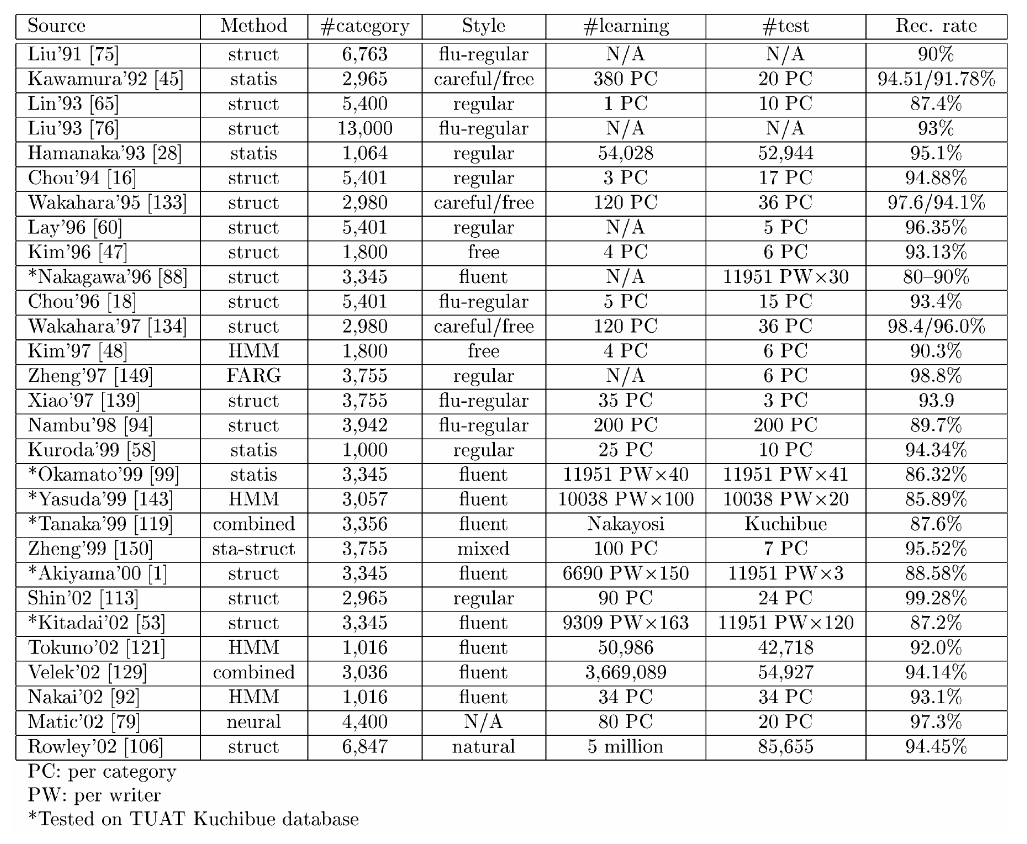
\includegraphics[scale=0.6]{images/recognitionRatesLiuJaeger.png}
    \caption{Recognition rates reported in the literature}
    \label{fig:recognitionratesreported}
  \end{center}
\end{figure}

\section{E-Learning Module Evaluation}
\label{sec:eval:elearning}
Generally, there are two main directions in the evaluation methodology
for e-learning applications: the educationalist's approach and the 
software developer's approach.
Therefore, the evaluation of an e-learning system is a complex task
and requires optimisation work on the account of both the conceptual
designer of an e-learning application as well as the software developer.

The e-learning part of the prototype is a sample module that is used 
to exemplify one usage scenario of the HWR engine. 
It mainly shows plausibility of the approach. A detailed analysis of the
e-learning application using ISO9126~\shortcite{Chua2004} is not useful,
since the e-learning part of the software has not been optimised in any way.
The focus of the thesis is not to implement an e-learning application,
but to create an analytical handwriting recognition engine.
It might be a prospect for future 
work\footnote{See section~\ref{sec:conclusion:newresearchpossibilities}}
to optimise the e-learning part and build a fully-developed e-learning
application for Japanese characters, but that would be outside the scope of 
this thesis. For these reasons, there will not be an evaluation of the
e-learning module.

\section{Evaluation of the HWR Engine}
\label{sec:eval:hwreval}

\subsection{General Considerations for Evaluation}
\label{sec:eval:generalconsiderations}

The performance of a recognition system can be measured in terms of speed,
accuracy and memory requirement.
While statistical systems offer high speed, 
but have large requirements on memory,
structural methods have lower speed, but require only a smaller 
memory~\shortcite{LiuJaegerNakagawa2004}.
The system developed and evaluated in this thesis is a structural system.
It can be expected that the system has a relatively low performance speed,
but moderate memory requirements. 
Additionally, since the system is not just a structural, but an analytical
recognition system, the speed might be even lower.

The factors memory requirements and speed are not of great interest in
the context of this system. The system is an on-line system, but it
exclusively performs single character recognition. The focus lies a lot more on
a detailed analysis of one character, rather than the high-speed recognition
of a stream of characters. The system is an interactive system. 
The recognition of a single character is an in-depth analysis of the
structure of that character and returns a profound feedback to the user.
Especially in an interactive learning context, the user is supposed to
work with the system's feedback. Recognition speed is interesting for evaluation
if the user enters a stream of characters. In that case recognition speed
can be expressed as a factor that relates recognition speed with input speed.
\shortciteANP{Tappert1990}~\citeyear{Tappert1990} state that on-line
recognition systems need only be fast enough to keep up with the writing. 
Further, they report average writing rates of  1.5-2.5  characters/s  for 
English  alphanumerics  and 0.2-2.5  characters/s  for  Chinese  characters.  
In a system that performs single character recognition the user has the 
impression of instant recognition.

Memory requirements are negligible in this system for a similar reason.
The recognition of one character does not require much memory compared to
the recognition of a stream of characters. Additionally, the main system engine
does not run on a small mobile computing device with low memory capacity,
but runs as a service on a standard PC. With the advanced memory capacities
of today memory is not an issue. Nevertheless, even mobile devices are 
equipped with enough memory to enable the system to perform analytical character
recognition.

For the reasons given above, the evaluation of the analytical handwriting 
recognition engine will be limited to different types of accuracy measurements.

\subsection{Development of Appropriate Evaluation Metrics}
\label{sec:eval:developmentofevalmetrics}

\subsubsection{Choice of Evaluation Subjects}
\label{sec:eval:evaluationsubjects}
It is difficult to perform an accuracy evaluation of a recognition system
that can be compared to other systems. The methods the systems use in order
to perform their recognition are diverse. There is always a trade-off between
robustness, performance and accuracy.
The prototype that is subject to this evaluation performs a different
task than most of the other recognition systems. It analyses the characters
not only for the purpose of recognition, but attempts to create feedback on
how well the input matched the character model in structural terms.
\begin{figure}[htbp]
  \begin{center}
    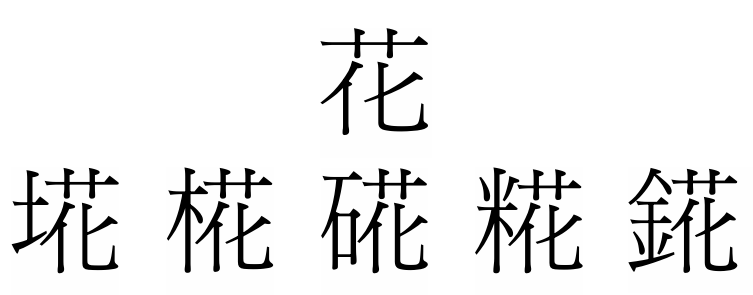
\includegraphics[scale=0.4]{images/simlarCharaters.png}
    \caption{Similar characters that can be confusing to learners: Five different Kanji share the same Radical in the \emph{tsukuri} position (on the right).}
    \label{fig:similarcharactersforuserconfusion}
  \end{center}
\end{figure}
That means concretely, the system can analyse an input with an expected result
and can perform the same for an unknown input by assuming the best match
as the expected result. The analysis yields an output that includes more
information than pure pattern matching. It rather includes structural linguistic 
information.

For example, the characters 
\cjk{埖}, \cjk{椛}, \cjk{硴}, \cjk{糀} and \cjk{錵} all share the substructure
on the right: \cjk{花}.
Figure~\ref{fig:similarcharactersforuserconfusion} shows the
substructure on top and below five characters that are using the structure.
The system analyses and distinguishes substructures. If the system is set
up to recognise an input with an expected result the output contains
a confidence value about the input quality concerning that character.
Additionally, the error recognition module returns information about the
substructures that were found in the input.
The similarity of the characters from 
figure~\ref{fig:similarcharactersforuserconfusion} is known to
the recognition system because of the identical substructures.
If the system identifies the input as a character with identical parts
with respect to the expected character the output will contain the information
as a substructure confusion error type.

This detailed analysis creates a unique requirement for evaluation. Not only
recognition accuracy must be measured and compared to other systems,
but a new evaluation for the recognition of substructures is needed.
It seems reasonable to measure the recognition accuracy in a plain 
percentage of correctly recognised characters. 
Precision and recall are the correct measurement for the error recognition,
where characters with incorrect substructures should be analysed. 
That way, true positives, false positives, 
true negatives and false negatives can be distinguished.
Since the system can recognise pure substructures as well, it would 
be interesting to see the accuracy of a Radical recognition.

The lexicon is a sample lexicon that contains 50 characters. That circumstance
has to be kept in mind when comparing the evaluation results to other
systems. Creating a lexicon entry for a single character is a laborious task.
It would be outside the scope of the thesis to create a large lexicon.
Nevertheless, the characters have been chosen by graphic and
semantic criteria in order to create more possibilities for confusion.
There are many characters using the same key Radical, other characters
that simply look similar, which might evoke difficulties 
for both the learner and the system.
Three experiments will be conducted in order to evaluate the analytical
handwriting recognition engine:
\begin{enumerate}
  \item \textbf{Overall recognition accuracy} \label{eval:enum:overall}
  \item \textbf{Substructure recognition accuracy} \label{eval:enum:substructure}
  \item \textbf{Error recognition accuracy} \label{eval:enum:errorrecognition}
\end{enumerate}
The metrics details for these experiments will be presented in the following 
sections.

\subsubsection{Overall Recognition Accuracy}
\label{sec:eval:overallrecognitionaccuracy}

The overall recognition accuracy (experiment~\ref{eval:enum:overall}) will 
be calculated as a measure of the \(n\)-best matches for a character input. 
\(N\) is defined as the lowest position in the list of \(n\)-best matches 
that will still be considered as a \emph{match} of a character. 
That is, if \(N\) is set to \(1\), then only the best match will be considered.
If \(N = 3\), the best three matches will be taken into account.
The overall recognition accuracy \(A_{N}\) is defined here as the weighted 
percentage of correctly recognised characters when taking the \(N\) best 
matches into account. The number of samples will be called \(S\).
\(r\) is an integer that marks the position in the list of \(n\)-best matches.
The values for \(r\) that will be considered for the evaluation lie 
on the open interval \(]1,N[\). If an input produces a confidence value 
for a character recognition high enough to be in a list position \(r \leq N\), 
then \(\frac{1}{r}\) will be added to the number of correctly 
recognised characters.
That means, if a character is the best match in the list of \(n\)-best matches,
then it is ranked on top, therefore \(r = 1\). 
Hence, \(\frac{1}{r} = \frac{1}{1} = 1\) will be added to the number of 
correct matches. If the correct character is the second best match, 
\(\frac{1}{2}\) will be added and so forth. If the input has been correctly 
recognised as the \(r\)-best match, but \(r > N\) or, alternatively,
the input has not been recognised at all, nothing will be added. 
\(f\) is a helper function that returns a value
according to the relation between \(r\) and \(N\). The variable
\(r_{i}\) denotes the position of the \(i^{\text{th}}\) input character in
the list of \(n\)-best matches for that input sequence and character. \(r_{i}\) serves as an input
value for \(f\). \(A_N\) will be calculated as follows:
\begin{quote}
  \(
    f(r, N):=
    \begin{cases}
      \frac{1}{r} & \quad \text{if $r \leq N$} \\
      0 & \quad \text{if $r > N$}
    \end{cases}
  \)
\end{quote}
\begin{quote}
  \(
    A_N := \frac{1}{S} \cdot \sum\limits_{i=1}^{S}{f(r_{i},N)}
  \)
\end{quote}\label{eval:accuracycalculation}
An example for the application of that term would be to set \(N = 1\).
Only the best match will be considered for an input.
If 100 input sequences are tested, then \(S=100\). 
If, for example, one of the \(S_{i}\) input sequences yields a high 
confidence value for the character the sequence is supposed to represent and 
the character becomes the most salient in the list of best matches
and occupies the first position. Then \(r_{i} = 1\) and \(f(r_{i},N) = f(1,1)\) 
yields \(1\).
Therefore, in the summation of all the \(f(r_{i},N)\) the value \(1\) 
will be added for each correctly recognised character.
Say, \(69\) of the \(100\) input characters were correctly recognised,
then \(A_{N} = A_{1} = \frac{1}{100} \cdot 69\). That would equal a 
result of \(69\%\). The key to this evaluation method is of course the 
value of \(N\). Multiple experiments with different \(N\)-values will be 
conducted for best comparability.

\paragraph{Baseline.} Different possibilities exist for the definition of a 
baseline for that experiment. A baseline based on pure randomness would 
be \(\frac{1}{C}\) with \(C\) representing the number of characters 
in the database. 
For \(C = 50\) the baseline would then be \(\frac{1}{C} = \frac{1}{50} = 0.02\).
That is already a very low baseline. The larger the lexicon grows the
lower the baseline for evaluation. For a lexicon that contains around 2,000 
characters and covers the Jōyō Kanji the baseline would come down to
\(\frac{1}{C} = \frac{1}{2000} = 0.0005\).
This baseline is certainly not sufficient to measure the quality of a 
recognition system. However, a significant baseline can be defined 
with the formula for the computation of \(A_N\) and generous assumptions
about the accuracy of the recognition: \\
Assume, \(N = 3\) and all the sample characters are among the first three 
matches in the list of matches, equally partitioned.
Then one third would yield \(r = 1\) with \(f(r,N)=f(1,3)=1\),
another third yield \(r = 2\) with \(f(r,N)=f(2,3)=\frac{1}{2}\),
and the last third yield \(r = 3\) with \(f(r,N)=f(3,3)=\frac{1}{3}\).
That leads to a baseline (\(B\)) calculation as follows:
\begin{quote}
  \(
    B := \frac{1}{S} \cdot (\sum\limits_{i=1}^{\frac{S}{3}}{f(1,3)} + \sum\limits_{i=1}^{\frac{S}{3}}{f(2,3)} + \sum\limits_{i=1}^{\frac{S}{3}}{f(3,3)}) \\
       = \frac{1}{S} \cdot (\sum\limits_{i=1}^{\frac{S}{3}}{1} + \sum\limits_{i=1}^{\frac{S}{3}}{\frac{1}{2}} + \sum\limits_{i=1}^{\frac{S}{3}}{\frac{1}{3}}) \\
       = \frac{1}{S} (\frac{S}{3} + \frac{S}{3 \cdot 2} + \frac{S}{3 \cdot 3}) 
       = \frac{1}{3} + \frac{1}{6} + \frac{1}{9}
       = \frac{11}{18} = 0.61
  \)
\end{quote}
The baseline value of \(0.61\) will be used for the overall recognition accuracy
experiment.

\subsubsection{Substructure Recognition Accuracy}
\label{sec:eval:substructurerecognitionaccuracy}

The substructure recognition accuracy (experiment~\ref{eval:enum:substructure}
will be measured in a similar way as the overall recognition accuracy.
In fact the same metrics will be used. See the previous section for details
on the metrics. The accuracy \(A_{N}\) will be measured as a percentage value
of correct recognition results, where the recognition as second-best or 
third-best (generally n-best, with \(n>1\)) will be devaluated. %xxx \emph{devaluate}?!? \textbf{abwerten}, \textbf{weniger gewichten}, \emph{nicht} komplett \textbf{entwerten}! xxx
This reduction of value is expressed mathematically by using the multiplicative 
inverse \(r^{-1}\) of the rank \(r\) in the list of \(n\)-best 
matches as a summand for the weighted sum of correct recognitions.
The equations for calculating the accuracy have been given in 
section~\ref{sec:eval:overallrecognitionaccuracy}
on page~\pageref{eval:accuracycalculation}.

The main difference is that many substructures occur in more than one 
character. In order to account for a substructure recognition will be regarded 
as \emph{correct}, if the input yields the intended substructure from
one of the characters that contain the substructure.
That fairly generous interpretation of what is correct considers the fact
that the substructures should be recognised for any of the characters.
During the recognition process it does not matter, what character needs to be
recognised the substructure recognition should work independently.
In a future version of the database the substructures should be stored only once
and then be shared among all characters that contain it.
The \emph{baseline} for the substructure recognition will be \(0.61\), 
the same number and using the same line of argument from 
section~\ref{sec:eval:overallrecognitionaccuracy}.

\subsubsection{Error Recognition Accuracy}
\label{sec:eval:errorrecognitionaccuracy}

The error recognition accuracy (experiment~\ref{eval:enum:errorrecognition}) 
is more difficult to evaluate than the pure accuracy.
The question arises, what kind of errors are expected to be found
and what kind of error corrections should be provided.
Error recognition here means that the system compares a known character with 
a given input stroke sequence. The input can contain flaws that do not 
represent the character appropriately. The prototype is expected to find the flaw
and propose a correction.
The evaluation method will be a classical \emph{precision and recall} method.
There are two possible cases in the input stroke sequence:
\begin{itemize}
  \item There is an error in the input with respect to the desired character.
  \item There is no error in the input.
\end{itemize}
There are two possibilities for the system to react:
\begin{itemize}
  \item The system identifies an error in the input with respect to the desired
        character and gives feedback on that error.
  \item The system does not identify an error in the input with respect to the
        desired character.
\end{itemize}
Those possibilities yield a \(2 \times 2\)-matrix:
Table~\ref{table:eval:resultsforprecisionandrecall} gives an overview about 
the possible results combined with the reality of the sample.

\begin{table}[htbp]
\begin{center}
  \begin{tabular}{|l|l|l|p{200pt}|}
    \hline
                           & Error in input      & No error in input \\
    \hline
    Found error (TP+FP)    & true positive (TP)  & false positive (FP) \\
    \hline
    No error found (FN+TN) & false negative (FN) & true negative (TN) \\
    \hline
  \end{tabular}
\end{center}
\caption{Possible results as a basis for precision and recall analysis.}
\label{table:eval:resultsforprecisionandrecall}
\end{table}
The precision \(P\) and recall \(R\) of the error recognition are computed 
with the standard formulae:
\begin{quote}
\(
P=tp \cdot (tp+fp)^{-1} \\
R=tp \cdot (tp+fn)^{-1} \\
\)  
\end{quote}
Additionally, the \emph{F-measure} will be used, however only for an equally 
important interpretation of precision and recall. Therefore, \(\beta = 1\) will
be fixed:
\begin{quote}
\(
F_{\beta} = (1 + \beta^2) \cdot \frac{P \cdot R }{ \beta^2 \cdot P + R} \\
F_{1} = 2 \cdot \frac{P \cdot R }{P + R} \\
\)
\end{quote}

\subsection{Experimental Results}
\label{sec:eval:experimentalresults}

Having presented the experimental metrics in the previous sections, 
the experimental results and the conclusions drawn will be presented in this 
section.

\subsubsection{Overall Recognition Accuracy Results}
\label{sec:eval:resultsoverallrecognition}

For the experiment concerning the overall recognition accuracy two test writers 
wrote all 50 characters from the database as an input sequence for the system.
That process yielded 100 input stroke sequences.
The input was stored in order for the experiment to be repeated without
physically re-entering the characters. Five sample characters from each 
writer haven been removed from the test set for detailed analysis.
With five characters from each writer in the development set, there were 
90 characters for the test set.
The test set characters have been used only for testing, not for 
detailed analyses. The development set characters have been tested as well
and the recognition process as well as the recognition result have been 
examined in order to improve the recognition engine.

The final evaluative run of the test set has been repeated 10 times, 
with different values for \(N\). All of the integers from 1 to 10 have
been used. The \emph{weighted number of recognised characters} (WNCR) changes 
according to the number of characters recognised in each rank in the
list of \(n\)-best matches. Table~\ref{table:eval:overallrecognitionresults}
shows the results in greater detail. With each incrementation of \(N\),
that is with decreasing strictness the recognition results rise.
The range of the weighted accuracy results goes from 70\% for \(N=1\) 
up to 81\% for \(N=5\). Taking into account even greater ranks up 
to \(N = 10\) in the list of \(n\)-best matches increased the result slightly
to 82\%. This development can also be seen in the chart in 
figure~\ref{fig:eval:overallrecognitionresults}.
\begin{table}[htbp]
\begin{center}
  \begin{tabular}{|c|c|c|c|c|c|c|c|c|c|c|c|c|p{200pt}|}
    \hline
N & A_N  &WNRC/90&  1 & 2 & 3 & 4  & 5 & 6 & 7 & 8 & 9 & 10 \\
    \hline
1 & 0.70 & 63.00 & 63 & - & - & -  & - & - & - & - & - & -  \\
    \hline
2 & 0.74 & 67.00 & 63 & 8 & - & -  & - & - & - & - & - & -  \\
    \hline
3 & 0.77 & 69.33 & 63 & 8 & 7 & -  & - & - & - & - & - & -  \\
    \hline
4 & 0.80 & 71.83 & 63 & 8 & 7 & 10 & - & - & - & - & - & -  \\
    \hline
5 & 0.81 & 72.63 & 63 & 8 & 7 & 10 & 4 & - & - & - & - & -  \\
    \hline
6 & 0.81 & 72.80 & 63 & 8 & 7 & 10 & 4 & 1 & - & - & - & -  \\
    \hline
7 & 0.81 & 73.23 & 63 & 8 & 7 & 10 & 4 & 1 & 3 & - & - & -  \\
    \hline
8 & 0.82 & 73.35 & 63 & 8 & 7 & 10 & 4 & 1 & 3 & 1 & - & -  \\
    \hline
9 & 0.82 & 73.58 & 63 & 8 & 7 & 10 & 4 & 1 & 3 & 1 & 2 & -  \\
    \hline
10& 0.82 & 73.68 & 63 & 8 & 7 & 10 & 4 & 1 & 3 & 1 & 2 & 1  \\
    \hline
  \end{tabular}
\end{center}
\caption{Overall recognition results.}
\label{table:eval:overallrecognitionresults}
\end{table}
\begin{figure}[htbp]
  \begin{center}
    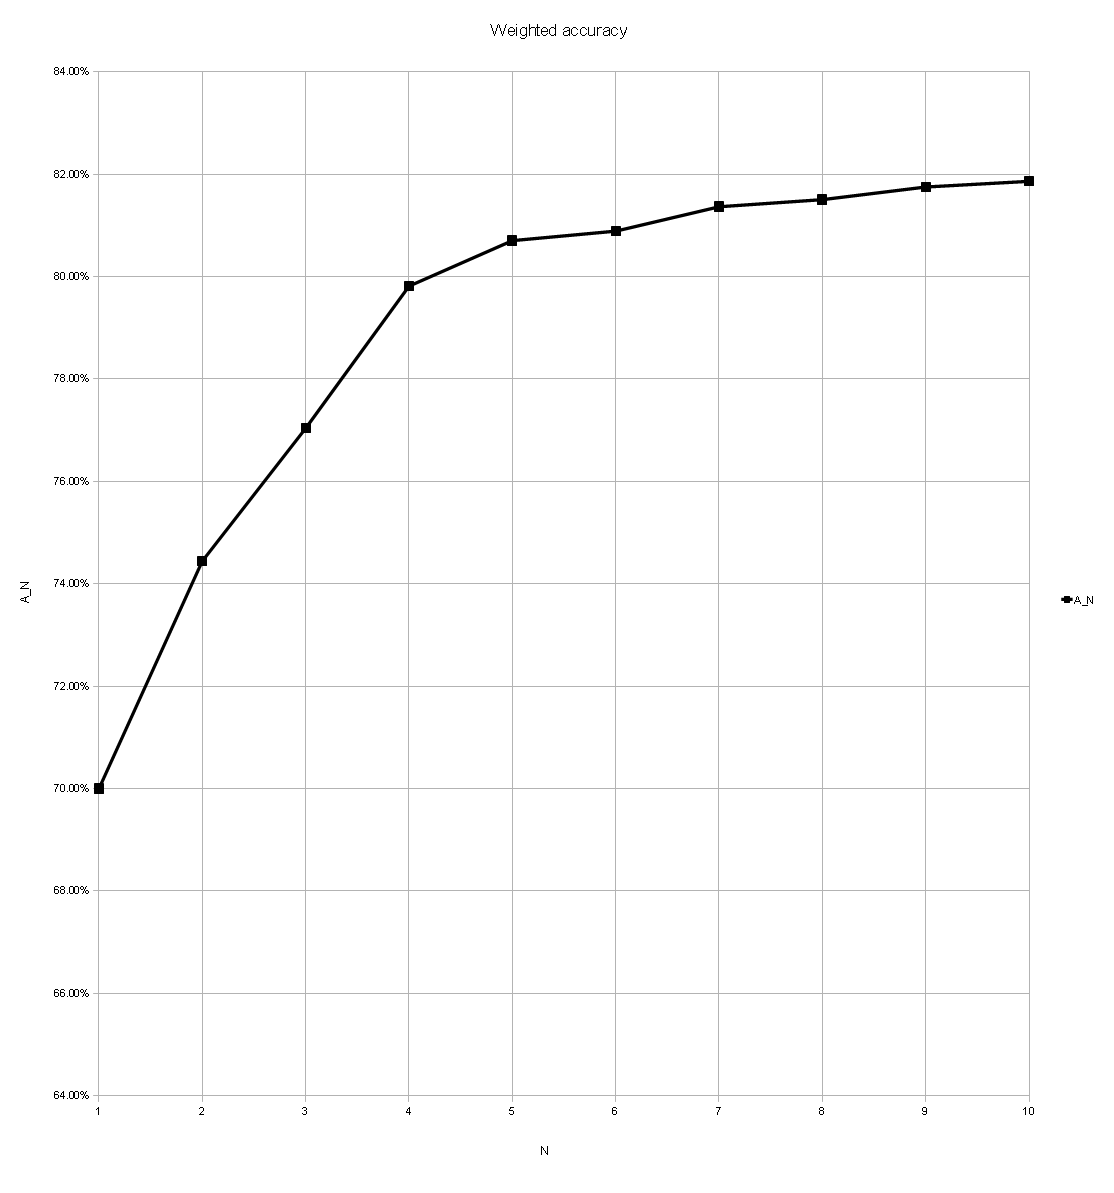
\includegraphics[scale=0.5]{images/weightedAccuracyOverall.png}
    \caption{Overall recognition results chart}
    \label{fig:eval:overallrecognitionresults}
  \end{center}
\end{figure}

\paragraph{Result Interpretation.}
As mentioned earlier, the characters bear a lot of potential for confusion,
since many of the database characters have been chosen by their key Radical
or by similar graphical appearance to other characters already in the database.
That special choice of characters seems to explain why there is such an
increase in accuracy when more ranks are taken into account.
The similar characters will be confused by the system and appear in
the lower ranks (higher \(r\)-values) in the list of \(n\)-best matches.
Even though all the results, even the one with \(N = 1\) are sizeably above
the baseline of 61\%.
Generally, the accuracy results are considerably lower than those of other
systems (see section~\ref{sec:eval:othersystems}). 
However, it has to be noted that the aim of this system is not 
to provide a handwriting recognition highly optimised for speed and accuracy.
Hence, there is little comparability for these results. 
The prototype of the analytical handwriting recognition fulfils an additional 
task that the other systems do not aim at. That obviously leads to a trade-off
concerning pure recognition performance.
The aim is to create a deep analysis of a character structure and
be able to provide feedback on the input. These abilities of the system will
be evaluated in the following sections.

The analysis of recognition errors among the development set characters 
revealed that there are two main types of errors: 
\begin{enumerate}
\item \textbf{Different stroke order}\label{eval:strokeordererrortype}
\item \textbf{Similar characters}    \label{eval:similarcharactererrortype}
\item \textbf{Segmentation ambiguity}\label{eval:segmentationambiguityerrortype}
\end{enumerate}
The type~\ref{eval:strokeordererrortype} and 
type~\ref{eval:similarcharactererrortype} errors errors probably occur for
all handwriting systems, but especially for overlaid or continuous handwriting.
Those types of error might be resolved if the recognition engine
was using a statistical model like a \emph{Hidden Markov Model.}
The segmentation ambiguity is a problem that occurs in overlaid handwriting
recognition for full characters. In analytical handwriting recognition
the problem occurs for substructures. The beginning and the end
of a substructure can only be found by completely analysing the substructure,
the previous and the following substructure. That process has
shown to be time-consuming.

\subsubsection{Substructure Recognition Accuracy Results}
\label{sec:eval:resultssubstructurerecognition}
For the evaluation of the recognition of substructures it would have been
desirable to use the same input data with which the overall evaluation
had been conducted. That was not possible, because it would have required
to analyse the input data and split it into substructures manually.
The input data for the evaluation of the substructures has been provided by
three writers each of whom entered 25 substructures, i.e.\ a total of 75
Radicals and Graphemes. That means 75 different tokens, not 75 different types.
Each type has only been written once by each writer.
This input set is a pure test set it has not been split or used for
development work. The results of the substructure recognition evaluation
might be more comparable to the results of other system.
The metrics for the substructure recognition are essentially the same as for
the overall evaluation.
The difference is that only the first three entries in the \(n\)-best list
will be considered. The structures are smaller, need less analysis, do not
have further substructures except the individual strokes. 
As expected, the evaluation results are higher than those of the overall 
recognition accuracy. The general trend can be seen in 
figure~\ref{fig:eval:substructurerecognitionresults}, the complete data is
laid out in table~\ref{table:eval:substructurerecognitionresults}.

\begin{table}[htbp]
\begin{center}
  \begin{tabular}{|c|c|c|c|c|c|p{200pt}|}
    \hline
N &  A_N & WNRC/75&  1 & 2 & 3 \\
    \hline
1 & 0.85 & 64     & 64 & - & - \\
    \hline
2 & 0.89 & 67     & 64 & 6 & - \\
    \hline
3 & 0.90 & 67.33  & 64 & 6 & 1 \\
    \hline
  \end{tabular}
\end{center}
\caption{Substructure recognition results.}
\label{table:eval:substructurerecognitionresults}
\end{table}

\begin{figure}[htbp]
  \begin{center}
    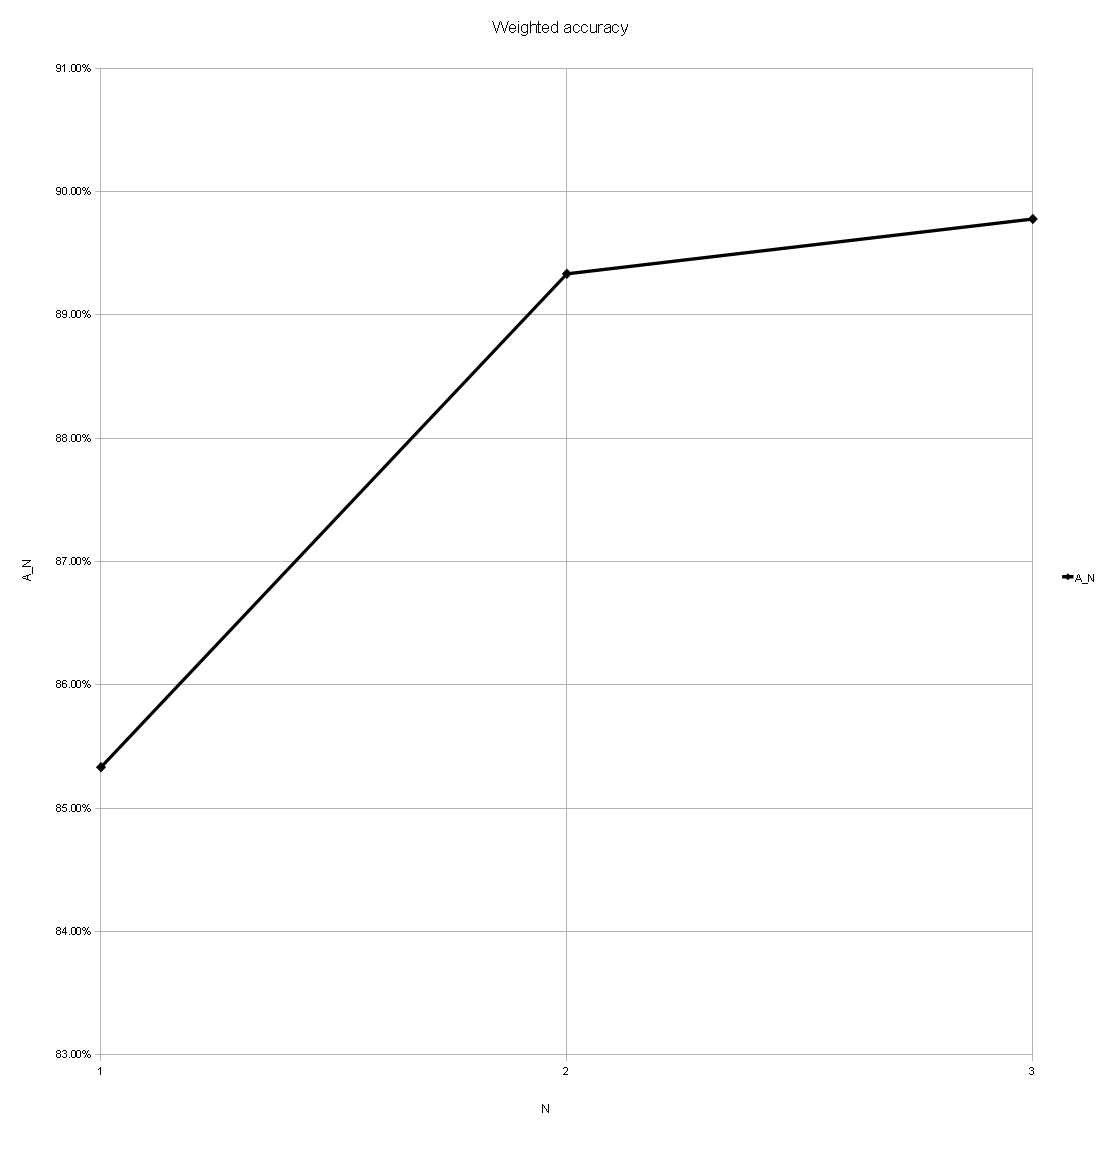
\includegraphics[scale=0.5]{images/weightedAccuracySubstructures.png}
    \caption{Substructure recognition results chart}
    \label{fig:eval:substructurerecognitionresults}
  \end{center}
\end{figure}

\paragraph{Result Interpretation.}
As expected, the accuracy of the recognition results for the substructures
was higher than the overall character recognition accuracy.
The substructure recognition is more robust as it does not have a segmentation
problem. Each input sequence is known to be a full substructure. 
During the recognition process the database needs to be searched for 
substructures. If a matching structure is found the process is completed.
The same pattern like in overall recognition accuracy can be observed 
concerning the lower positions in the list of \(n\)-best matches.


\subsubsection{Error Recognition Accuracy Results}
\label{sec:eval:resulterrorrecognition}

The error recognition evaluation required more manual work than the overall 
recognition or substructure recognition evaluation. This is due to the fact
that errors had to be produced intelligently in order for the error recognition
to pick them up. Therefore, this evaluation type has to be seen more as a 
qualitative analysis, rather than a pure quantitative evaluation.

\paragraph{Test Data Creation.}
One writer created 30 characters, including 20 characters with errors,
i.e.\ 20 characters where one Radical had been replaced with another one
or with garbled input. Figure~\ref{fig:eval:botsuumiprintvsdrawn} shows the
characters~\cjk{没} (Jap.\ pron.\ \emph{botsu}; Eng.\ 'to sink') %935
and~\cjk{海} (Jap.\ pron.\ \emph{umi}; Eng.\ 'sea') %117
both in print and handwritten versions.
The two characters share the same key Radical. It is the 'water'-Radical 
on the left side (marked in red). 
On the right side, the lower Radical is fairly distinct
and therefore no cause of confusion. In fact~\cjk{海}~(umi/'sea') contains the 
'mother'-Radical~\cjk{母} (marked in purple), 
while~\cjk{没}~(botsu/'to sink') contains the 
'again'-Radical~\cjk{又} (marked in purple), 
which looks very similar to the 
'father'-Radical~\cjk{父} (not contained in the figure).
This mother/father-analogy has nothing to do with the true meaning
of the characters, it can just serve as a mnemonic for a learner.
This fact could be a cause for semantic confusion due to the 
mnemonic trick, but clearly those two Radicals offer little features 
for a graphical confusion between the two.
The upper Radical on the right in both characters is a small two-stroke
Radical that can easily be confused graphically with another small two-stroke 
Radical (marked in green). This danger of confusion exists both for a human
and for the character recogniser. 
Non-existent blended characters like the one shown in 
figure~\ref{fig:eval:hybrid935and117} have been created as erroneous input
for the error recognition evaluation test set.
\begin{figure}[htbp]
  \begin{center}
    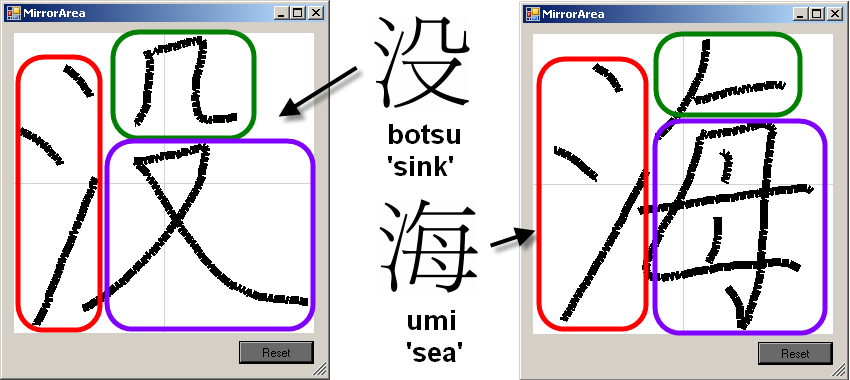
\includegraphics[scale=0.75]{images/char935vsChar117HandwrittenMarked.png}
    \caption{Characters \cjk{没} (\emph{botsu}, 'sink') and \cjk{海} (\emph{umi}, 'sea')}
    \label{fig:eval:botsuumiprintvsdrawn}
  \end{center}
\end{figure}
In case of a confusion of the two Radicals in the upper right corner of 
the character the user might produce an input like the one in 
figure~\ref{fig:eval:hybrid935and117}.
\begin{figure}[htbp]
  \begin{center}
    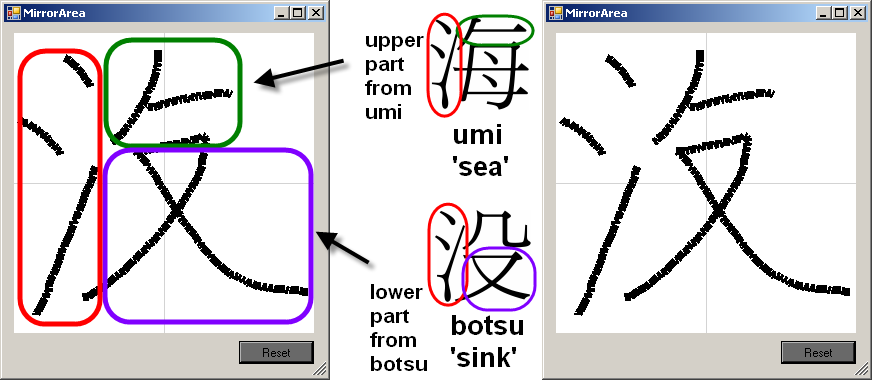
\includegraphics[scale=0.57]{images/char935and117HybridMarked.png}
    \caption{Confusion between the characters \cjk{没} (\emph{botsu}, 'sink') and \cjk{海} (\emph{umi}, 'sea')}
    \label{fig:eval:hybrid935and117}
  \end{center}
\end{figure}

\paragraph{Error Recognition Result Data Set.}
Table~\ref{table:eval:resultsprecisionandrecallnumbers} shows the results 
of the error recognition test run. 
In section~\ref{sec:eval:errorrecognitionaccuracy} it has been argued that the
correct evaluation method for the error recognition was a precision and recall
measurement.
\begin{table}[htbp]
\begin{center}
  \begin{tabular}{|l|l|l|p{200pt}|}
    \hline
    Total of 30 chars (20/10) & Error in input      & No error in input \\
    \hline
    16 found error (TP+FP)    & 14 (TP)             & 2 (FP) \\
    \hline
    9 no error found (FN+TN)  & 6 (FN)              & 3 (TN) \\
    \hline
    5 unrecognised (?)        & 3 (?)               & 2 (?) \\
    \hline
  \end{tabular}
\end{center}
\caption{Error recognition results as a basis for precision and recall analysis.}
\label{table:eval:resultsprecisionandrecallnumbers}
\end{table}
The problem with a pure precision and recall analysis is that the results
in table~\ref{table:eval:resultsprecisionandrecallnumbers} are not 2-way, 
but 3-way. The error recognition engine returned the three result sets 
\emph{character contains error}, \emph{characters does not contain error}
and \emph{character could not be recognised}.
Now the question arises whether the unrecognised characters should be 
regarded as incorrect or correct. 
If there was an error in the input character and the character could 
not be recognised, this could be regarded as a \emph{true positive}.
If no recognition is possible that could mean there is an error in 
the character, therefore an error has been found.
However, that is just an interpretation of the results and
would increase the error recognition performance undeservedly. 
On the other hand, if the input was a correct character,
then assuming the result to be an error message would add 
to the number of \emph{false positives}, 
lowering the performance result of the error recognition.
The error recognition is a sub-component of the character recognition engine,
it cannot work independently from it. 
Hence, either way it would be an unfair to include the unrecognised
characters into the evaluation of the error recognition.

In order to ensure a fair evaluation, but also in order to provide 
a result set qualified for a 2-way evaluation, the unrecognised characters are 
exempt from the evaluation of the error recognition.
Table~\ref{table:eval:resultsprecisionandrecallnumbersunrecognisedexempt}
shows the data set that was used for the calculation of precision and recall
without the unrecognised characters. The total input set consisted of 30 characters, 20 with errors in the characters, 10 correct characters.
After exempting the unrecognised characters from the evaluation there is a total
of 25 characters, 17 of which containing errors, 8 correct characters.
\begin{table}[htbp]
\begin{center}
  \begin{tabular}{|l|l|l|p{200pt}|}
    \hline
    Total of 25 chars (17/8)  & Error in input      & No error in input \\
    \hline
    16 found error (TP+FP)    & 14 (TP)             & 2 (FP) \\
    \hline
    9 no error found (FN+TN)  & 6 (FN)              & 3 (TN) \\
    \hline
  \end{tabular}
\end{center}
\caption{Error recognition results excluding the unrecognised characters as a
basis for a 2-way precision and recall analysis.}
\label{table:eval:resultsprecisionandrecallnumbersunrecognisedexempt}
\end{table}

\paragraph{Result Interpretation.}
The precision \(P\) and recall \(R\) can be computed from the values given in 
table~\ref{table:eval:resultsprecisionandrecallnumbersunrecognisedexempt}.
Precision:
\begin{quote}
\(
P=tp \cdot (tp+fp)^{-1} \\
= 14 \cdot (14+2)^{-1} \\
= 0.875
\)
\end{quote}
Recall:
\begin{quote}
\(
R=tp \cdot (tp+fn)^{-1} \\
=14 \cdot (14+6)^{-1} \\
=0.7
\)  
\end{quote}
Additionally, the \emph{F-measure} will be used, however only for an equally 
important interpretation of precision and recall. Therefore, \(\beta = 1\) will
be fixed:
\begin{quote}
\(
F_{1} = 2 \cdot \frac{P \cdot R }{P + R} \\
 = 2 \cdot \frac{0.875 \cdot 0.7 }{0.875 + 0.7} \\
 = 0.78
\)
\end{quote}
The results are difficult to interpret because there are no other systems for 
comparison that perform a similar analytical handwriting recognition.
Precision is slightly below 90\%, meaning if an error had been recognised,
it had been recognised correctly most of the times.
That is valuable for the sample application the e-learning environment.
The number of falsely detected errors is low.
The recall is not impressively high, 
but well above the obvious 50\% baseline for a 2-way precision calculation,
that would result from a random assignment of \emph{error} or \emph{no error}
to all characters in the test set.

\section{Conclusions}
\label{sec:eval:conclusions}

In this chapter, the evaluation of the handwriting recognition engine has 
been presented. The overall recognition had an accuracy of 70\%-82\%.
That is below highly optimised recognition system and shows the trade-off that
had to be taken in order to perform a detailed internal analysis of the 
characters.
The recognition of substructures had better results, the accuracy lied around
85\%-90\%. That value is more comparable to other recognition systems that do
not perform a detailed analysis of substructures.
The error recognition showed a satisfying result of 87.5\% precision at a recall 
rate of 70\%.
The next chapter of the thesis draws overall conclusions from the work.